\documentclass[11pt,reqno]{amsart}
\usepackage{amsfonts,amsmath,amssymb,amsbsy,amstext,amsthm,mathtools}
\usepackage{accents,color,enumerate,enumitem,float,fullpage,verbatim}

\usepackage[margin=1.0049in,includeheadfoot]{geometry}

\usepackage{url}
%\usepackage[colorlinks=true,hyperindex, linkcolor=magenta, pagebackref=false, citecolor=cyan,draft]{hyperref}
\usepackage[nolinks=true]{hyperref}

%\usepackage[alphabetic]{amsrefs} 

%\usepackage{eucal,bm,kpfonts,mathbbol}
\usepackage[dvipsnames]{xcolor}

\usepackage{tikz,tikz-cd}	
\usetikzlibrary{positioning, matrix, shapes}         								    				
\usetikzlibrary{arrows,calc,matrix}

\usepackage{lscape}

\usepackage{microtype}


\usepackage{titlesec}		
\setcounter{secnumdepth}{4}						     					% Allows one to use nice section titles
\titleformat{\section}[block]{\scshape\bfseries\filcenter}{\thesection.}{1em}{}		% Creates section titles
\titleformat{\subsection}[runin]{\scshape\bfseries}{\thesubsection}{1em}{}			% Creates subsection titles
\titleformat{\subsubsection}[runin]{\scshape\bfseries}{\thesubsubsection}{1em}{}			% Creates subsection titles

\usepackage[titles]{tocloft}								     					% Creates table of fancy contents
\setcounter{tocdepth}{4}
\renewcommand{\contentsname}{}	     					% Renames and centers title of ToC

\usepackage{multirow}
\usepackage{array}
\usepackage{booktabs}
\newcolumntype{M}[1]{>{\centering\arraybackslash}m{#1}}
\newcolumntype{N}{@{}m{0pt}@{}}
\usepackage{diagbox}
\usepackage{cancel}

\newtheorem{lemma}{Lemma}[section]
\newtheorem{theorem}[lemma]{Theorem}
\newtheorem{goalTheorem}[lemma]{Goal Theorem}
\newtheorem{goal}[lemma]{Research Goal}
\newtheorem{problem}[lemma]{Research Problem}
\newtheorem{prop}[lemma]{Proposition}
\newtheorem{cor}[lemma]{Corollary}
\newtheorem{conjecture}[lemma]{Conjecture}
\newtheorem{claim}[lemma]{Claim}
\newtheorem{defn}[lemma]{Definition} 
\newtheorem{notation}[lemma]{Notation} 
\newtheorem{exercise}[lemma]{Exercise}
\newtheorem{question}[lemma]{Question}
\newtheorem*{assumption}{Assumption}
\newtheorem{principle}[lemma]{Principle}
\newtheorem{heuristic}[lemma]{Heuristic}

\newtheorem{theoremalpha}{Theorem}
\newtheorem{corollaryalpha}[theoremalpha]{Corollary}
\renewcommand{\thetheoremalpha}{\Alph{theoremalpha}}

\theoremstyle{remark}
\newtheorem{remark}[lemma]{Remark}
\newtheorem{example}[lemma]{Example}
\newtheorem{cexample}[lemma]{Counterexample}

% Commands
\newcommand{\initial}{\operatorname{in}}
\newcommand{\NF}{\operatorname{NF}}
\newcommand{\HF}{\operatorname{HF}}
\newcommand{\Hilb}{\operatorname{Hilb}}
\newcommand{\depth}{\operatorname{depth}}
\newcommand{\reg}{\operatorname{reg}}
\newcommand{\Span}{\operatorname{span}}
\newcommand{\img}{\operatorname{img}}
\newcommand{\inn}{\operatorname{in}}

\newcommand{\length}{\operatorname{length}}
\newcommand{\coker}{\operatorname{coker}}
\newcommand{\adeg}{\operatorname{adeg}}
\newcommand{\pdim}{\operatorname{pdim}}
\newcommand{\Spec}{\operatorname{Spec}}
\newcommand{\Ext}{\operatorname{Ext}}
\newcommand{\Tor}{\operatorname{Tor}}
\newcommand{\LT}{\operatorname{LT}}
\newcommand{\im}{\operatorname{im}}
\newcommand{\NS}{\operatorname{NS}}
\newcommand{\Frac}{\operatorname{Frac}}
\newcommand{\Khar}{\operatorname{char}}
\newcommand{\Proj}{\operatorname{Proj}}
\newcommand{\id}{\operatorname{id}}
\newcommand{\Div}{\operatorname{Div}}
\newcommand{\Kl}{\operatorname{Cl}}
\newcommand{\tr}{\operatorname{tr}}
\newcommand{\Tr}{\operatorname{Tr}}
\newcommand{\Supp}{\operatorname{Supp}}
\newcommand{\ann}{\operatorname{ann}}
\newcommand{\Gal}{\operatorname{Gal}}
\newcommand{\Pic}{\operatorname{Pic}}
\newcommand{\QQbar}{{\overline{\mathbb Q}}}
\newcommand{\Br}{\operatorname{Br}}
\newcommand{\Bl}{\operatorname{Bl}}
\newcommand{\Kox}{\operatorname{Cox}}
\newcommand{\conv}{\operatorname{conv}}
\newcommand{\getsr}{\operatorname{Tor}}
\newcommand{\diam}{\operatorname{diam}}
\newcommand{\Hom}{\operatorname{Hom}} %done
\newcommand{\sheafHom}{\mathcal{H}om}
\newcommand{\Gr}{\operatorname{Gr}}
\newcommand{\rank}{\operatorname{rank}} 
\newcommand{\codim}{\operatorname{codim}}
\newcommand{\Sym}{\operatorname{Sym}} %done
\newcommand{\GL}{{GL}}
\newcommand{\Prob}{\operatorname{Prob}}
\newcommand{\Density}{\operatorname{Density}}
\newcommand{\Syz}{\operatorname{Syz}}
\newcommand{\pd}{\operatorname{pd}}
\newcommand{\supp}{\operatorname{supp}}
\newcommand{\cone}{\operatorname{\textbf{cone}}}
\newcommand{\Res}{\operatorname{Res}}
\newcommand{\HS}{\operatorname{HS}}
\newcommand{\Cl}{\operatorname{Cl}}
\newcommand{\oO}{\operatorname{O}}

\newcommand{\defi}[1]{\textsf{#1}} % for defined terms

\newcommand{\remd}{\operatorname{remd}}
\newcommand{\colim}{\operatorname{colim}}
\newcommand{\trideg}{\operatorname{tri.deg}}
\newcommand{\indeg}{\operatorname{index.deg}}
\newcommand{\moddeg}{\operatorname{mod.deg}}
\newcommand{\Desc}{\operatorname{Desc}}
\newcommand{\inter}{\operatorname{int}}
\newcommand{\Nef}{\operatorname{Nef}}
\newcommand{\Jac}{\operatorname{Jac}}
\newcommand{\Cox}{\operatorname{Cox}}
\newcommand{\GKZ}{\operatorname{gkz}}

\newcommand{\gon}{\operatorname{gon}}
\newcommand{\cliff}{\operatorname{Cliff}}

\newcommand{\doot}{\bullet}

\newcommand{\Alt}{\bigwedge\nolimits}
\newcommand{\Set}{\text{\bf Set}}										% Category of Sets
\newcommand{\Sch}{\text{\bf Sch}}										% Category of Abelian Groups
\newcommand{\Mod}[1]{\ (\mathrm{mod}\ #1)}




%%%%%%%%%%%%%%%%%%%%%%%%%%%%%% Letters  %%%%%%%%%%%%%%%%%%%%%%%%%%%%%%%%%%%%%%%%%%%%
%%%%%%%%%%%%%%%%%%%%%%%%%%%%%%%%%%%%%%%%%%%%%%%%%%%%%%%%%%%%%%%%%%%%%%%%%%%%%%%
\renewcommand{\aa}{\mathbf{a}}
\newcommand{\dd}{\mathbf{d}}
\newcommand{\nn}{\mathbf{n}}
\newcommand{\ee}{\mathbf{e}}
\newcommand{\ff}{\mathbf{f}}
\newcommand{\vv}{\mathbf{v}}
\newcommand{\ww}{\mathbf{w}}
\newcommand{\one}{\mathbf{1}}
\newcommand{\pp}{\mathbf{p}}
\newcommand{\qq}{\mathbf{q}}

\renewcommand{\AA}{\mathbb{A}}
\newcommand{\BB}{\mathbb{B}}
\newcommand{\CC}{\mathbb{C}}
\newcommand{\DD}{\mathbb{D}}
\newcommand{\EE}{\mathbb{E}}
\newcommand{\FF}{\mathbb{F}}
\newcommand{\GG}{\mathbb{G}}
\newcommand{\HH}{\mathbb{H}}
\newcommand{\II}{\mathbb{I}}
\newcommand{\JJ}{\mathbb{J}}
\newcommand{\KK}{\mathbb{K}}
\newcommand{\LL}{\mathbb{L}}
\newcommand{\MM}{\mathbb{M}}
\newcommand{\NN}{\mathbb{N}}
\newcommand{\PP}{\mathbb{P}}
\newcommand{\QQ}{\mathbb{Q}}
\newcommand{\RR}{\mathbb{R}}
\renewcommand{\SS}{\mathbb{S}}
\newcommand{\TT}{\mathbb{T}}
\newcommand{\UU}{\mathbb{U}}
\newcommand{\VV}{\mathbb{V}}
\newcommand{\WW}{\mathbb{W}}
\newcommand{\XX}{\mathbb{X}}
\newcommand{\YY}{\mathbb{Y}}
\newcommand{\ZZ}{\mathbb{Z}}


\newcommand{\cA}{\mathcal{A}}
\newcommand{\cB}{\mathcal{B}}
\newcommand{\cC}{\mathcal{C}}
\newcommand{\cD}{\mathcal{D}}
\newcommand{\cE}{\mathcal{E}}
\newcommand{\cF}{\mathcal{F}}
\newcommand{\cG}{\mathcal{G}}
\newcommand{\cH}{\mathcal{H}}
\newcommand{\cI}{\mathcal{I}}
\newcommand{\cJ}{\mathcal{J}}
\newcommand{\cK}{\mathcal{K}}
\newcommand{\cL}{\mathcal{L}}
\newcommand{\cM}{\mathcal{M}}
\newcommand{\cN}{\mathcal{N}}
\newcommand{\cO}{\mathcal{O}}
\newcommand{\cP}{\mathcal{P}}
\newcommand{\cQ}{\mathcal{Q}}
\newcommand{\cR}{\mathcal{R}}
\newcommand{\cS}{\mathcal{S}}
\newcommand{\cT}{\mathcal{T}}
\newcommand{\cU}{\mathcal{U}}
\newcommand{\cV}{\mathcal{V}}
\newcommand{\cW}{\mathcal{W}}
\newcommand{\cX}{\mathcal{X}}
\newcommand{\cY}{\mathcal{Y}}
\newcommand{\cZ}{\mathcal{Z}}

\DeclareMathOperator{\RB}{RB}
\DeclareMathOperator{\Trop}{Trop}
\DeclareMathOperator{\trop}{Trop}

\DeclareMathOperator{\OO}{O}
\DeclareMathOperator{\SL}{SL}
\DeclareMathOperator{\Sp}{Sp}
\DeclareMathOperator{\Ag}{\mathcal{A}_{g}}
\DeclareMathOperator{\PDrt}{PD^{rt}}
\DeclareMathOperator{\PD}{PD}
\DeclareMathOperator{\Herm}{Herm}

\newcommand{\juliette}[1]{{\color{red} \sf $\spadesuit\spadesuit\spadesuit$ Juliette: [#1]}}

\newcommand{\kit}[1]{{\color{blue} \sf Kit: [#1]}}
\newcommand{\jcite}{{\color{blue} \sf $\heartsuit\heartsuit\heartsuit$:cite}}

%%%%%%%%%%%%%%%%%%%%%%%%%%%%%%%%%%%%%%%%%%%%%%%%%%%%%%%%%%%%%%%%%%%%%%%%%%%%%%%

\title{Project Description: Multigraded Homological Algebra and Geometry}

%%%%%%%%%%%%%%%%%%%%%%%%%%%%%%%%%%%%%%%%%%%%%%%%%%%%%%%%%%%%%%%%%%%%%%%%%%%%%%%

\begin{document} 
\thispagestyle{empty}
\pagestyle{empty}
\begingroup  
  \centering
  \large\scshape\bfseries Project Description: Multigraded Homological Algebra and Geometry\\[1em]
\endgroup

%\tableofcontents

\setcounter{section}{0}

\noindent This proposal involves research in algebraic geometry and commutative algebra with several connections to computation and combinatorics, as well as a wide array of broader impacts.
% Additionally, it includes a wide array of broader impacts. As an overview: 
\begin{itemize}[leftmargin=*]
	\item \S~\ref{sec:prior-work} \textbf{Results of Prior NSF Support.} 
	\item \S~\ref{sec:syzygies-on-stacks} \textbf{The Geometry of Multigraded Syzygies on Stacks}
	\item \S~\ref{sec:multigraded-regularity} \textbf{Castelnuovo–Mumford Regularity: Resolutions, Bounds, and Asymptotics}
	\item \S~\ref{sec:uniform-homological-algebra-on-toric} \textbf{Uniform Homological Algebra on Toric Varieties}
	\item \S~\ref{sec:broader-impacts} \textbf{Broader Impacts.}
\end{itemize}

%%%%%%%%%%%%%%%%%%%%%%%%%%%%%%%%%%%%%%%%%%%%%%%%%%%%%%%%%%%%%%%%%%%%%%%%%%%%%%%
%%%%%%%%%%%%%%%%%%%%%%%%%%%%%%%%%%%%%%%%%%%%%%%%%%%%%%%%%%%%%%%%%%%%%%%%%%%%%%%
\section{Results of Prior NSF Support}\label{sec:prior-work}
%%%%%%%%%%%%%%%%%%%%%%%%%%%%%%%%%%%%%%%%%%%%%%%%%%%%%%%%%%%%%%%%%%%%%%%%%%%%%%%
%%%%%%%%%%%%%%%%%%%%%%%%%%%%%%%%%%%%%%%%%%%%%%%%%%%%%%%%%%%%%%%%%%%%%%%%%%%%%%%

During 2020-2022 the PI was supported by an NSF Postdoctoral Research Fellowship (NSF Grant No. MSPRF DMS-2002239, \$150,000) titled \textit{Asymptotic Syzygies in Algebraic Geometry}. In this period the PI made major contributions to extending our understanding of homological algebra on toric varieties (see Section~\ref{subsec:prior:homological-algebra-on-toric}) and the cohomology of moduli spaces (see Section~\ref{subsec:prior:cohomology-of-ag}). These works resulted in 5 new papers being posted to the arXiv \cite{BCEGLY22,bruceHellerSayrafi21,bruceHellerSayrafi22,brandtBruceCorey23,BBCMMW24}.

During 2015-2020 the PI was supported by an NSF Graduate Research Fellowship (NSF Grant No. DGE-1256259, \$150,000) title \textit{Syzygies in Algebraic Geometry}. In this period the PI made substantial contributions to commutative algebra and algebraic geometry, including furthering our understanding of syzygies on higher dimensional varieties. This resulted in the PI posting 8 new papers to the arXiv \cite{ABLS20,BBBKR17,bruceErman19,bruceLi20,BEGY20,BEGY21,bruce24,bruce22}.

Of the 12 new papers the PI posted to the arXiv during these periods of support 9 of these above-mentioned papers were accepted for publication, including in such journals as \textit{Algebra \& Number Theory} \cite{bruceErman19}, \textit{Geometry \& Topology} \cite{BBCMMW24}, \textit{Journal of Algebra} \cite{BCEGLY22}, and \textit{Experimental Mathematics} \cite{BEGY20}. The PI contributed to 4 open-source software packages, one public-facing database, and two articles for the \textit{Notices of the AMS} \cite{BBB21,bruceNotices22}. A more detailed summary of these results and their intellectual merits continues in the following sections. 

%%%%%%%%%%%%%%%%%%%%%%%%%%%%%%%%%%%%%%%%%%%%%%%%%%%%%%%%%%%%%%%%%%%%%%%%%%%%%%%
\subsection{Asymptotic Syzygies}
%%%%%%%%%%%%%%%%%%%%%%%%%%%%%%%%%%%%%%%%%%%%%%%%%%%%%%%%%%%%%%%%%%%%%%%%%%%%%%%

Broadly, asymptotic syzygies is the study of the graded Betti numbers (i.e. the syzygies) of a projective variety as the positivity of the embedding grows. For a smooth projective variety $X\subset \PP^{n_{d}}$ embedded by a very ample line bundle $L_{d}$, following \cite{ermanYang18}, set,
\begin{align*}
\rho_q\left(X,L_{d}\right)\;\;\coloneqq&\ \;\; \frac{\#\left\{p\in\NN |\; \big| \; \beta_{p,p+q}\left(X,L_{d}\right)\neq0\right\}}{n_{d}},
\end{align*}
which is the percentage of non-zero syzygies appearing in a row $q$ of the Betti table \cite[Theorem~1.1]{eisenbud05}. The asymptotic perspective asks how $\rho_{q}(X;L_{d})$ behaves along the sequence of line bundles $(L_{d})_{d\in \NN}$. In this language, Green's work on the syzygies of high degree curves can be phrased as follows.
\begin{theorem}\cite{green84-I}
Let $X\subset \PP^n$ be a smooth projective curve. If $(L_{d})_{d\in\NN}$ is a sequence of very ample line bundles on $X$ such that $\deg L_{d} = d$ then $\lim_{d\to \infty} \rho_{2}\left(X;L_{d}\right) = 0$.
\end{theorem}

Put differently, asymptotically the syzygies of curves are as simple as possible, occurring in the lowest possible degree. Ein and Lazarsfeld established the opposite asymptotic behavior for higher dimensional varieties under the analogous positivity condition. 

\begin{theorem}\cite[Theorem~C]{einLazarsfeld12}
Let $X\subset \PP^n$ be a smooth projective variety, $\dim X \geq2$, and fix an index $1\leq q \leq \dim X$. If $(L_{d})_{d\in\NN}$ is a sequence of very ample line bundles such that $L_{d+1}-L_{d}$ is constant and ample then $\lim_{d\to\infty} \rho_{q}\left(X; L_d\right) = 1$.
\end{theorem}

My work weakens the ample-growth hypothesis to semi-ample growth, recall a line bundle $L$ is \textit{semi-ample} if $|kL|$ is base point free for $k\gg0$ (e.g.  $\cO(1,0)$ on $\PP^{n}\times \PP^{m}$). I established the following asymptotic nonvanishing result for $PP^{n}\times\PP^{m}$ embedded by $\cO(d_{1},d_{2})$. 

\begin{theorem}\cite[Corollary~B]{bruce24}\label{thm:bruce-semiample}
Let $X=\PP^{n}\times\PP^{m}$ and fix an index $1\leq q \leq n+m$. There exist constants $C_{i,j}$ and $D_{i,j}$ such that
\[
\rho_{q}\left(X; \cO\left(d_1,d_2\right)\right)\geq1-\sum_{\substack{i+j=q \\  i \leq n, \; j \leq m}}\left(
\frac{C_{i,j}}{d_1^id_2^j}+\frac{D_{i,j}}{d_1^{n-i}d_2^{m-j}}\right)-O\left(\begin{matrix}\text{lower ord.}\\ \text{terms}\end{matrix}\right).
\]
\end{theorem}

If both $d_{1}\to \infty$ and $d_{2}\to\infty$ then $\rho_{q}\left(\PP^{n}\times\PP^{m}; \cO(d_1,d_2)\right)\to1$, recovering the results of Ein and Lazarsfeld for $\PP^n\times\PP^m$. However, if $d_{1}$ is fixed and $d_{2}\to \infty$ (i.e. semi-ample growth) my results bound the asymptotic percentage of non-zero syzygies away from zero. In fact I conjecture that, unlike in previously studied cases, in the semi-ample setting $\rho_{q}\left(\PP^{n}\times\PP^{m}; \cO(d_1,d_2)\right)$ does not approach 1. Proving this would require a vanishing result for asymptotic syzygies, which is open even in the ample case  \cite[Conjectures~7.1,~7.5]{einLazarsfeld12}.



%%%%%%%%%%%%%%%%%%%%%%%%%%%%%%%%%%%%%%%%%%%%%%%%%%%%%%%%%%%%%%%%%%%%%%%%%%%%%%%
%%%%%%%%%%%%%%%%%%%%%%%%%%%%%%%%%%%%%%%%%%%%%%%%%%%%%%%%%%%%%%%%%%%%%%%%%%%%%%%
\subsection{Eisenbud-Goto on Products of Projective Space}\label{subsec:prior:homological-algebra-on-toric}
%%%%%%%%%%%%%%%%%%%%%%%%%%%%%%%%%%%%%%%%%%%%%%%%%%%%%%%%%%%%%%%%%%%%%%%%%%%%%%%
%%%%%%%%%%%%%%%%%%%%%%%%%%%%%%%%%%%%%%%%%%%%%%%%%%%%%%%%%%%%%%%%%%%%%%%%%%%%%%%

The Castelnuovo–Mumford Regularity of a projective variety $X\subset \PP^{r}$ is a measure of the complexity of $X$ given in terms of the vanishing of certain cohomology groups of $X$. Roughly speaking one should think about Castelnuovo--Mumford regularity as being a numerical measure of geometric complexity. Eisenbud and Goto showed that regularity is also closely connected to interesting homological properties.

\begin{theorem}\cite{eisenbudGoto84}\label{thm:eisenbud-goto}
Let $\cF$ be a coherent sheaf on $\PP^{n}$ and $M=\bigoplus_{e\in\ZZ} H^0(\PP^{r},\cF(e))$ the corresponding section module. The following are equivalent: (1) $M$ is $d$-regular; (2) $\beta_{p,q}(M)=0$ for all $p\geq0$ and $q>d+i$; (3) $M_{\geq d}$ has a linear resolution. 
\end{theorem}

A toric variety $Y$ is a ``nice'' compactification of a torus, which under minor hypotheses can be thought of as the quotient $[(\CC^{n}\setminus \VV(B))/(\CC^{\times})^r]$ where $\VV(B)$ is the fixed locus of the action of $(\CC^{\times})^r$ on $\CC^{n}$. The ideal $B$ defining this fixed locus is called the irrelevant ideal, and when $Y\cong \PP^n$ it is precisely the maximal homogenous ideal $\langle x_0,\ldots,x_n\rangle$. Cox proved a beautiful correspondence between coherent sheaves on $Y$ and $\ZZ^r$-graded modules over a $\ZZ^r$-graded polynomial ring $S=\CC[x_0,\ldots,x_n]$, which is known as the Cox ring of $Y$. This suggests there may be a rich dictionary between \emph{multigraded} homological algebra over the Cox ring and geometry of the toric variety. 

Maclagan and Smith introduced multigraded Castelnuovo--Mumford regularity on toric varieties; defined in terms of the vanishing of cohomology groups,  Let $Y$ be a smooth projective toric variety, the Picard group of $Y$ is isomorphic to $\ZZ^r$ and the cone of numerically effective line bundles on $Y$ -- the nef cone of $X$ -- is a full dimensional cone of $\Pic(Y)\cong \ZZ^r$.  We define multigraded regularity in terms of vanishing of higher cohomology groups with respect to translates of this cone. Given $\vv \in \ZZ^r$ set $|\vv|\coloneqq v_1+v_2+\cdots v_r$. 

\begin{defn}\cite[Definition 6.1]{maclaganSmith04}\label{def:mg-reg}
With the set-up as in the previous paragraph if $\cF$ is a coherent module on $X$ then we say that $\cF$ is \emph{$\dd$-regular} for $\dd \in \ZZ^r$ if and only if $H^i(Y, \cF(\ee))=0$ for all $i>0$ and all $\ee \in L_{i}(\dd)$ where
\[
L_{i}(\dd) \coloneqq \bigcup_{\substack{\vv\in \ZZ^r \\ |\vv|=i}} \left(\dd-\vv + \Nef(X)\right).
\]
We then define the \emph{multigraded regularity} of $\cF$ to be $\reg(\cF)\coloneqq \{\dd\in \ZZ^r \;\; | \;\; \text{$\cF$ is $\dd$-regular}\}$. 
\end{defn}

\begin{center}
\begin{figure}[H]
\newcommand{\makegrid}{
  \path[use as bounding box] (-3.45,-3.25) rectangle (5.45,5.25);
  \foreach \x in {-4,...,4}
  \foreach \y in {-4,...,4}
    { \fill[Gray,fill=gray] (\x,\y) circle (1.5pt); }
  \draw[-,  semithick] (-4,0)--(4,0);
  \draw[-,  semithick] (0,-4)--(0,4);
}
%%%%%%%%%%%%%%%%%%%%%%%%%%%%%%%%%%%%
%%%%%%%%%%%%%%%%%%%%%%%%%%%%%%%%%%%%
%%%%%%%%%%%%%%%%%%%%%%%%%%%%%%%%%%%%
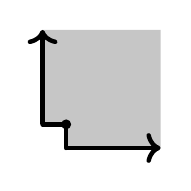
\begin{tikzpicture}[scale=.3]
  \path[fill=Gray!45] (-1,4)--(-1,0)--(0,0)--(0,-1)--(4,-1)--(4,4)--(-1,4);
  \makegrid
  \draw[->, ultra thick] (-1,0)--(-1,4);
  \draw[-, cap=round,ultra thick] (-1,0)--(0,0)--(0,-1);
    \draw[->, ultra thick] (0,-1)--(4,-1);
  %\fill[Gray,fill=Gray] (-1,0) circle (6pt);
 % \fill[Gray,fill=Gray] (0,-1) circle (6pt);
  \fill[Gray,fill=Black] (0,0) circle (6pt);
\end{tikzpicture}\quad\;
%%%%%%%%%%%%%%%%%%%%%%%%%%%%%%%%%%%%
%%%%%%%%%%%%%%%%%%%%%%%%%%%%%%%%%%%%
%%%%%%%%%%%%%%%%%%%%%%%%%%%%%%%%%%%%
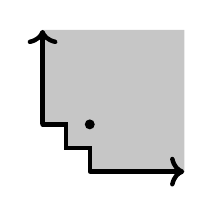
\begin{tikzpicture}[scale=.3]
  \path[fill=Gray!45] (-2,4)--(-2,0)--(-1,0)--(-1,-1)--(0,-1)--(0,-2)--(4,-2)--(4,4)--(-2,4);
  \makegrid
  \draw[->, ultra thick] (-2,0)--(-2,4);
  \draw[-, cap=round,ultra thick] (-2,0)--(-1,0)--(-1,-1)--(0,-1)--(0,-2);
    \draw[->, ultra thick] (0,-2)--(4,-2);
%  \fill[Gray,fill=Gray] (-2,0) circle (6pt);
 % \fill[Gray,fill=Gray] (-1,-1) circle (6pt);
 % \fill[Gray,fill=Gray] (0,-2) circle (6pt);
  \fill[Gray,fill=Black] (0,0) circle (6pt);
\end{tikzpicture}\quad\;
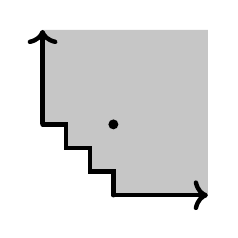
\begin{tikzpicture}[scale=.3]
  \path[fill=Gray!45] (-3,4)--(-3,0)--(-2,0)--(-3,0)--(-2,0)--(-2,-1)--(-1,-1)--(-1,-2)--(0,-2)--(0,-3)--(4,-3)--(4,4)--(-2,4);
  \makegrid
  \draw[->, ultra thick] (-3,0)--(-3,4);
  \draw[-, cap=round,ultra thick] (-3,0)--(-2,0)--(-2,-1)--(-1,-1)--(-1,-2)--(0,-2)--(0,-3);
      \draw[->, ultra thick] (0,-3)--(4,-3);
%  \fill[Gray,fill=Gray] (-2,0) circle (6pt);
 % \fill[Gray,fill=Gray] (-1,-1) circle (6pt);
 % \fill[Gray,fill=Gray] (0,-2) circle (6pt);
  \fill[Gray,fill=Black] (0,0) circle (6pt);
\end{tikzpicture}
%
\caption{The regions $L_{1}(0,0)$, $L_{2}(0,0)$, and $L_{3}(0,0)$ for $Y=\PP^n\times \PP^m$, in which case $\Pic(Y)\cong \ZZ^2$ and $\Nef(Y)$ is the first quadrant.}
\end{figure}
\end{center}

We can define the multigraded regularity of a $\ZZ^r$-graded module $M$ over $S$ in terms of analogous vanishing of local cohomology modules $H_{B}^I(M)$ where $B$ is the irrelevant ideal of $Y$. The multigraded Castelnuovo--Mumford regularity of is not a single number, but an infinite subset of $\ZZ^{r}$. 

The obvious approaches to generalize Theorem~\ref{thm:eisenbud-goto} to a product of projective spaces fail For example, the multigraded Betti numbers do not determine multigraded Castelnuovo--Mumford regularity \cite[Example 5.1]{bruceHellerSayrafi21}. Despite this we show that part (3) of Theorem~\ref{thm:eisenbud-goto} can be generalized. To do so we introduce the following generalization of linear resolutions. 

\begin{defn}
A complex $F_{\bullet}$ of $\ZZ^{r}$-graded free $S$-modules is $\dd$-quasilinear if and only if $F_{0}$ is generated in degree $\dd$ and each twist of $F_{i}$ is contained in $L_{i-1}(\dd-\one)$.
\end{defn}

\begin{theorem}\cite[Theorem A]{bruceHellerSayrafi21}\label{thm:mgreg-main}
Let $M$ be a (saturated) finitely generated $\ZZ^{r}$-graded $S$-module:
\[
\text{$M$ is $\dd$-regular} \iff  \text{$M_{\geq\dd}$ has a $\dd$-quasilinear resolution}.
\]
\end{theorem}

The proof of Theorem~\ref{thm:mgreg-main} is based on a spectral sequence argument relating the Betti numbers of $M_{\geq\dd}$ to the Fourier--Mukai transform of $\widetilde{M}$ with Beilinson's resolution of the diagonal as the kernel. This result provides an effective way to compute whether a module is regular at a given multidegree $\dd \in \ZZ^r$ and construct so called ``short virtual resolutions'' on products of projective spaces. 

%%%%%%%%%%%%%%%%%%%%%%%%%%%%%%%%%%%%%%%%%%%%%%%%%%%%%%%%%%%%%%%%%%%%%%%%%%%%%%%
\subsection{Asymptotic Multigraded Regularity of Ideals}
%%%%%%%%%%%%%%%%%%%%%%%%%%%%%%%%%%%%%%%%%%%%%%%%%%%%%%%%%%%%%%%%%%%%%%%%%%%%%%%

Building upon our work discussed above -- and inspired by previous work on $\PP^{r}$ \cite{BEL91,CHT99,Kodiyalam00} -- my collaborators and I also studied the asymptotic regularity of powers of ideals on arbitrary toric varieties. In particular, Definition~\ref{def:mg-reg} can be extended to all toric varieties by letting $S$ be Cox ring of the toric variety $X$, replacing $\ZZ^r$ with the Picard group of $X$, and replacing $\NN^{r}$ with the nef cone of $X$. My collaborators and I show that the multigraded regularity of powers of ideals is bounded and translates in a predictable way. In particular, the regularity of $I^{t}$ essentially translates within $\Nef X$ in fixed directions at a linear rate.
 

\begin{theorem}\cite[Theorem 4.1]{bruceHellerSayrafi22}
  There exists a degree $\aa\in\Pic X$, depending only on $I$, such that for each integer $t>0$ and each pair of degrees $\qq_1,\qq_2\in\Pic X$ satisfying $\qq_1\geq\deg f_i\geq\qq_2$ for all generators $f_i$ of $I$, we have
	\[ t\qq_1+\aa+\reg S \subseteq \reg\!\left(I^t\right) \subseteq t\qq_2+\Nef X. \]
\end{theorem}

%%%%%%%%%%%%%%%%%%%%%%%%%%%%%%%%%%%%%%%%%%%%%%%%%%%%%%%%%%%%%%%%%%%%%%%%%%%%%%%
\subsubsection{Syzygies via Highly Distributed Computing}
%%%%%%%%%%%%%%%%%%%%%%%%%%%%%%%%%%%%%%%%%%%%%%%%%%%%%%%%%%%%%%%%%%%%%%%%%%%%%%%

It is quite difficult to compute examples of syzygies. For example, until recently the syzygies of the projective plane embedded by the $d$-uple Veronese embedding were only known for $d\leq 5$. My co-authors and I exploited recent advances in numerical linear algebra and high-throughput high-performance computing to generate a number of new examples of Veronese syzygies. A follow-up project used similar computational approaches to compute the syzygies of $\PP^{1}\times\PP^{1}$ in over 200 new examples. This data provided support for several existing conjectures, as well as led us to make a number of new conjectures \cite{BEGY20,BCEGLY22}. 
The data is publicly available via SyzygyData.com and a package for Macaualy2 \cite{bruceErman19, M2}.


%%%%%%%%%%%%%%%%%%%%%%%%%%%%%%%%%%%%%%%%%%%%%%%%%%%%%%%%%%%%%%%%%%%%%%%%%%%%%%%
%%%%%%%%%%%%%%%%%%%%%%%%%%%%%%%%%%%%%%%%%%%%%%%%%%%%%%%%%%%%%%%%%%%%%%%%%%%%%%%
\subsection{Top-Weight Cohomology of $\mathcal{A}_{g}$}\label{subsec:prior:cohomology-of-ag}
%%%%%%%%%%%%%%%%%%%%%%%%%%%%%%%%%%%%%%%%%%%%%%%%%%%%%%%%%%%%%%%%%%%%%%%%%%%%%%%
%%%%%%%%%%%%%%%%%%%%%%%%%%%%%%%%%%%%%%%%%%%%%%%%%%%%%%%%%%%%%%%%%%%%%%%%%%%%%%%

The moduli space of (principally polarized) abelian varieties of dimension $g$, is a smooth variety $\cA_{g}$ (truthfully a smooth Delinge--Mumford stack) whose points are in one to one correspondence with isomorphism classes of principally polarized abelian varieties of dimension $g$. Concretely, we may view it as the quotient $[\mathbb{H}_g/\mathrm{Sp}(2g, \ZZ)]$ where $\HH_{g}$ is the Siegel upper half-space. Similar to the moduli space of curves $\cA_{g}$ has long been studied, but much remains unknown about its geometry. For example, the (singular) cohomology is $\cA_{g}$ is only fully known for $g\leq 4$ \cite{igusa62,hain02,HT12,HT18}. Further, Grushevsky \cite{grushevsky09} posed the question whether $H^{2k+1}(\cA_{g};\QQ)\neq0$ for some $g$ and $k$. Building upon the work of Chan, Galatius, and Payne \cite{CPG21}, my co-authors and I developed new methods for understanding a certain canonical quotient of the cohomology of $\cA_{g}$. In particular, our results construct non-trivial cohomology classes in $H^{k}(\cA_{g}; \QQ)$ in a number of new cases and answer Grushevsky's question. 

\begin{theorem}\cite[Theorem A]{BBCMMW24}\label{thm:Ag}
The rational cohomology $H^{k}\left(\cA_{g};\QQ\right)\neq0$ for:
\[
\text{$(g,k)=(5,15),(5,20),(6,30),(7,28),(7,33),(7,37)$, and $(7,42)$}.
\]
\end{theorem}

For broader context, since $\cA_g$ is a rational classifying space for $\mathrm{Sp}_{2g}(\ZZ)$ there is natural isomorphism $H^*(\cA_g;\QQ) \cong H^*(\mathrm{Sp}_{2g}(\ZZ);\QQ)$. In particular, the above results provide new non-vanishing results for $H^*(\mathrm{Sp}_{2g}(\ZZ);\QQ)$. However, my work takes advantage of the fact that since $\cA_g$  is a smooth and separated Deligne Mumford stack with a coarse moduli space which is an algebraic variety, permitting Deligne's mixed Hodge theory to be applied to study the rational cohomology of these groups. In this way we deduce Theorem~\ref{thm:Ag} above as a corollary to computing the top-weight cohomology of $\cA_{g}$ for all $g\leq 7$.  

%%%%%%%%%%%%%%%%%%%%%%%%%%%%%%%%%%%%%%%%%%%%%%%%%%%%%%%%%%%%%%%%%%%%%%%%%%%%%%%
%%%%%%%%%%%%%%%%%%%%%%%%%%%%%%%%%%%%%%%%%%%%%%%%%%%%%%%%%%%%%%%%%%%%%%%%%%%%%%%
\subsection{Broader Impacts from Prior NSF Support}
%%%%%%%%%%%%%%%%%%%%%%%%%%%%%%%%%%%%%%%%%%%%%%%%%%%%%%%%%%%%%%%%%%%%%%%%%%%%%%%
%%%%%%%%%%%%%%%%%%%%%%%%%%%%%%%%%%%%%%%%%%%%%%%%%%%%%%%%%%%%%%%%%%%%%%%%%%%%%%%

\subsubsection{Organizing}\label{subsubsec:prior-organizing} I organized 11 conferences: \textit{Math Careers Beyond Academia } (50 participants), \textit{M2@UW} (45 participants), \textit{Geometry \& Arithmetic of Surfaces} (40 participants), \textit{CAZoom} (70 participants), \textit{WAGS} (100 participants), \textit{Gems of Combinatorics I \& II} (40 \& 30 participants), $\Spec(\overline{\QQ})$ (50 participants), \textit{BATMOBILE (2022)} (20 participants),  \textit{Gems of Commutative Algebra I \& II} (35 \& 40 participants). In this time I organized three special sessions at AMS Sectional Meetings and the Joint Math Meetings. Many of these workshops, namely the \textit{Gems of} series, focused on supporting  the next generation of researchers by building community and networks.


\subsubsection{Math Circles}
	From 2015 through 2018 I was heavily involved in the Madison Math Circle, including  2 years as the lead organizer. As an organizer, I worked to build stronger connections between the Madison Math Circle, local schools, teachers, and other outreach organizations. This led to weekly attendance to more than double. I also created a new outreach arm of the circle, which visits high schools around the state of Wisconsin to better serve students. While a post-doc at UC Berkeley I volunteered as a speaker with the Berkeley Math Circle. 

\subsubsection{Mentoring}
I have actively sought out ways to mentor undergraduate and graduate students, especially those from generally underrepresented groups. While a graduate student, I led reading courses with three undergraduates. One of these students, an undergraduate woman, worked with me for over a year, during which time I helped her apply for summer research projects. Working with \textit{Girls' Math Night Out} I lead two girls in high school through a project exploring cryptography. During 2018-2019, I mentored 6 first-year graduate students (all women or non-binary students). I also mentored two undergraduate women via the AWM's Mentoring Network. 

I advised two summer research projects for undergraduate students. The first of these projects ran virtually during Summer 2021 when 6 undergraduates worked on combinatorial questions related to my work in \cite{BBCMMW24}. In Summer 2022 I advised an undergraduate student on a research project related to my work on syzygies discussed in Section~\ref{subsec:prior:homological-algebra-on-toric}. This student is now a graduate student in mathematics and received an NSF GRF. As a postdoc, I began research projects with three graduate students (a majority of whom identify with a generally underrepresented group). These projects have resulted in two pre-prints, with additional projects still ongoing. Throughout the Spring and Summer of 2022, I did a reading course with a first-year graduate woman on algebraic geometry.

\subsubsection{Virtual Mathematics}
In response to the COVID-19 pandemic and the shift of many mathematical activities to virtual formats, I worked to find ways for these online activities to reach those often at the periphery. During Summer and Fall 2020, I helped with Ravi Vakil's \textit{Algebraic Geometry in the Time of Covid} project. This massive online open-access course in algebraic geometry brought together $\sim2,000$ participants from around the world. In Spring 2021, I organized an 8-week virtual reading course for undergraduates in algebraic geometry and commutative algebra. 

%\subsubsection{t} 
%While a graduate student I co-founded oSTEM@UW as a resource for LGBTQ+ students in STEM, which eventually grew to over fifty active members. As one member said, ``It made me very happy to see other friendly LGBTQ+ faces around... Thanks so much for organizing this stuff -- it's really helpful''. From 2017-2020 I led the campus social organization for LGBTQ+ graduate and post-graduate students, which had over 350 members. 
%
%Since Fall 2020 I have organized \textit{Trans Math Day}, an annual one-day virtual conference promoting the work of transgender and non-binary mathematicians. Highlighting the importance of such conferences one student participant said, ``I've been really considering leaving mathematics.  [Trans Math Day 2020] reminded me why I'm here and why I want to stay. ... If a conference like this had been around for me five years ago, my life would have been a lot better.'' Trans Math Day regularly has ~50 participants. 
%
%During 2020-2023 I served as a board member for \textit{Spectra: The Association for LGBTQ+ Mathematicians}, including the inaugural president. I oversaw the growth and formalization of the organization, including the creation and adoption of bylaws, the creation of an invited lecture at the Joint Math Meetings, and a fundraising campaign that has raised over \$20,000.


%%%%%%%%%%%%%%%%%%%%%%%%%%%%%%%%%%%%%%%%%%%%%%%%%%%%%%%%%%%%%%%%%%%%%%%%%%%%%%%
%%%%%%%%%%%%%%%%%%%%%%%%%%%%%%%%%%%%%%%%%%%%%%%%%%%%%%%%%%%%%%%%%%%%%%%%%%%%%%%
\section{The Geometry of Multigraded Syzygies on Stacks}\label{sec:syzygies-on-stacks}
%%%%%%%%%%%%%%%%%%%%%%%%%%%%%%%%%%%%%%%%%%%%%%%%%%%%%%%%%%%%%%%%%%%%%%%%%%%%%%%
%%%%%%%%%%%%%%%%%%%%%%%%%%%%%%%%%%%%%%%%%%%%%%%%%%%%%%%%%%%%%%%%%%%%%%%%%%%%%%%

Let $X$ be a projective variety and $L$ a very ample line bundle. Considering the embedding of $X$ into projective space $X \hookrightarrow \PP H^{0}(X,L)\cong \PP^{n}$ defined by $L$, let $S_{X}=S/I_{X}$ where $S=\CC[x_{0},\ldots,x_{n}]$ is the standard graded polynomial ring and $I_{X}$ is the homogeneous defining ideal of $X$. The minimal graded free resolution of $S_{X}$ as an $S$-module is an exact sequence:
\begin{center}
\begin{tikzcd}[column sep = 3em]
0 & \lar{} S_{X} & \arrow[l,"\epsilon" above]  F_{0} & \arrow[l,"d_{1}" above] \cdots &  & \cdots & \arrow[l,"d_{k-1}" above]  F_{k-1} & \arrow[l,"d_{k}" above] F_{k} & \lar \cdots
\end{tikzcd}
\end{center}
where $F_{p}$ is a graded free $S$-module, and the differentials satisfy some minimality conditions. Since $F_{p}$ is a graded free $S$-module it can be written as $\bigoplus_{q}S(-q)^{\beta_{p,q}(S_{X})}$. The module $S(-q)$ is the ring $S$ with a twisted grading, so that $S(-q)_{d}$ is equal to $S_{d-q}$ where $S_{d-q}$ is the graded piece of degree $d-q$. The $\beta_{p,q}(S_{X})$ are known as the graded Betti numbers (or syzygies) of the pair $(X,L)$, and we often denote them as $\beta_{p,q}(X;L)$ to indicate their dependence not just on $X$ but on the line bundle $L$ as well. That is to say the syzygies depend on the extrinsic embedding of $X$ into $\PP^{n}$. An overarching theme in the study of syzygies in algebraic geometry is understanding ways that minimal graded free resolutions and grade Betti numbers also capture the intrinsic geometry of $X$.   

For example, Mumford's work on the geN

The connection between the geometry of $X$ and its minimal graded free resolutions has been made most precise when $X$ is a curve. This sec

 For example, consider the following classical theorem of Noether and Petri concerning canonical curves.

\begin{theorem}[Noether-Petri Theorem]\label{thm:noether-petri}
	Let $X$ be a smooth projective curve of genus $g$. If $X$ does not have a degree $2$ cover of $\PP^{1}$ then the canonical bundle $K_{X}$ defines a projectively normal embedding of $X$ into $\PP^{g-1}$. Further, if $X$ does not admit a degree 3 cover of $\PP^{1}$ then the image of $X\subset \PP^{g-1}$ is defined by quadrics. 
\end{theorem}

In the language of minimal graded free resolutions this theorem can be translated as follows: 
\begin{itemize}
\item If $X$ does not admit a cover of $\P^{1}$ of degree $2$ then $\beta_{0,0}(X;K_X)=1$ and $\beta_{0,q}(X;K_X)=0$ for all $q\neq0$. 
\item If $X$ does not admit a cover of $\P^{1}$ of degree $3$ then $\beta_{1,q}(X;K_X)=0$ for all $q\neq2$. 
\end{itemize}


%%%%%%%%%%%%%%%%%%%%%%%%%%%%%%%%%%%%%%%%%%%%%%%%%%%%%%%%%%%%%%%%%%%%%%%%%%%%%%%
\subsection{$N_{p}$-Conditions for Stacky Curves}
%%%%%%%%%%%%%%%%%%%%%%%%%%%%%%%%%%%%%%%%%%%%%%%%%%%%%%%%%%%%%%%%%%%%%%%%%%%%%%%


A \textit{stacky curve} is a smooth proper geometrically connected Deligne-Mumford stack of dimension 1 which contains a dense open subscheme. intuitively one may think about a stacky curve as being a curve with a finite number of special points -- called stacky points -- which have ``fractional degrees''. Note this intuition can be made precise in the sense that any stacky curve is (Zariski) locally the quotient of a smooth affine curve by a finite group \cite{voightZurieckBrown22}*{Lemma~5.3.10}. For simplicity we work over $\CC$, however, everything remains true over an arbitrary field if one places minor conditions on the stacky curve. 

In \cite{voightZurieckBrown22} Voight and Zureick-Brown develop a theory of line bundles, including canonical divisors, for stacky curves. Roughly this theory proceeds by noting that every stacky curve $\cX$ admits a coarse space $\pi:\cX\to X$ where $X$ is a smooth (non-stacky) curve. The theory of line bundles on $\cX$ can be developed by carefully transferring properties of divisors on $X$ to $\cX$ via the map $\pi$. The key thing to note is that since the degree of a stacky point need not be an integers the degree of a line bundle on a stacky curve maybe be a rational number. Associated to stacky curve $\cX$ and a line bundle $\cL$ the \emph{section module} of $\cX$ with respect to $\cL$ is $R(\cX;\cL)\coloneqq \bigoplus_{k\in \ZZ}H^{0}(\cX,k\cL)$. 

\begin{goal}
	Understand the syzygies of $R(\cX,\cL)$ where $\cX$ is a stacky curve and $\cL$ is a line bundle on $\cX$. 
\end{goal}

A fundamental difference between the the classical theory on varieties is that a line bundle $\cL$ on stacky curve does not define an embedding into projective space, instead it defines an embedding into we weighted projective stack. Algebraically this corresponds to the fact that $R(\cX;\cL)$ is a module over a polynomial ring with a non-standard $\ZZ$-grading. That is there exists a $\ZZ$-graded polynomial ring $S=\CC[x_{1},x_{2},\ldots,x_{n}]$ where $\deg(x_{i})=w_{i}\in\ZZ$ such that $R(\cX;\cL) \cong S/I$ for some homogeneous ideal $I\subset S$.

\begin{example}\label{example:canonical-ring}
Suppose $\cX$ is a stacky curve with two stacky points each having $\ZZ/2\ZZ$ as its stabilizer and whose coarse space has genus 1. The canonical ring of $\cX$ can be minimally presented as
\[
R(\cX;K_{\cX})\cong \CC[x_{1},x_{2},x_{3}]/\langle x_{3}^{2}x_{1}-bx_{3}x_{2}^{6}-x_{1}^{2}-ax_{2}^{8}\rangle
\]
where $a,b\in \CC$ and $\deg(x_{1})=4$, $\deg(x_{2})=1$, and $\deg(x_{3})=2$ \cite{voightZurieckBrown22}*{Remark 8.3.6}. 
\end{example}

\begin{problem}
	Let $\cX$ be a stacky curve with $e$ the maximum order of the stabilizer groups of stacky points on $\cX$. Let $\cL$ a line bundle on $\cX$. 
	\begin{enumerate}
	\item Find a characterization in terms of $\deg(\cL)$ for when $R(\cX:\cL)$ is Cohen-Macaulay.
	\item Find a characteriz in terms of $\deg(\cL)$ for when $R(\cX:\cL)$ is generated in degrees$\leq 2e$. 
	\end{enumerate}
\end{problem}

\begin{problem}
	Let $\cX$ be a stacky curve whose coarse space has genus 0 or 1. If $\cL$ is a line bundle on $\cX$ and $\deg(\cL)\gg0$, what $N_{p}$ conditions does $R(\cX; \cL)$ satisfy? Determine precise bounds on $\deg(\cL)$ guaranteeing $N_p$.
\end{problem}

\begin{example}[Weighted Projective Line]
Consider the stacky curve $\cX = \cP(1,e)$, the weighted projective line. Its coarse space is $\PP^1$. It has one stacky point with stabilizer $\ZZ/e\ZZ$. The coordinate ring corresponding to the ample generator of $\Pic(\cX)$ is $R = \KK[x,y]$, where $\deg(x)=1$ and $\deg(y)=e$. This is not standard graded. If we embed $\cX$ by a high degree line bundle $\cL$, the resulting ring $R(\cX;\cL)$ will be a Veronese subring of $\KK[x,y]$. The syzygies must be studied relative to the weights of the variables.
\end{example}

We will begin with the genus 0 case (weighted projective lines). We will adapt techniques from Koszul cohomology and the theory of kernel bundles (e.g., the $M_L$-type bundles used in the proof of Green's theorem) to the stacky setting. The Riemann-Roch theorem for stacky curves relates $h^0(\cX, \cL)$ to $\deg(\cL)$ and the orders $e_i$. We expect the bounds on $\deg(\cL)$ to depend explicitly on the $e_i$, likely involving the least common multiple of the orders.

For the genus 1 case, the geometry is richer. Stacky elliptic curves can be described as quotients of $\CC$ by a lattice and a finite group action. The PI plans to leverage techniques inspired by the work of Polishchuk on the Fourier-Mukai transform for elliptic curves, generalized to the equivariant setting, to analyze the stability and splitting types of the relevant kernel bundles.

%%%%%%%%%%%%%%%%%%%%%%%%%%%%%%%%%%%%%%%%%%%%%%%%%%%%%%%%%%%%%%%%%%%%%%%%%%%%%%%
\subsection{Green's Conjecture for Canonical Stacky Curves} 
%%%%%%%%%%%%%%%%%%%%%%%%%%%%%%%%%%%%%%%%%%%%%%%%%%%%%%%%%%%%%%%%%%%%%%%%%%%%%%%

One perspective on the Noether-Petri Theorem is that the syzygies of a smooth projective curve $X$ seem to be closely related to the degrees for which $X$ admits a cover of $\PP^{1}$. This heuristic turns out to be true in several ways, but to understand the higher syzygies of canonical curves one needs a slightly more subtle invariant. The Clifford index of a smooth curve $X$ is defined to be:
 \[
\cliff(X)\coloneqq \min \left\{\deg(L) - 2 \dim H^{0}(X,L)+2 \quad \bigg| \begin{matrix} L\in \Pic(X) \\
\deg(L)\leq g-1 \quad \dim H^0(X,L)\geq2\end{matrix}\right\}.
\]
As a vast generalization of the Noether-Petri theorem, the following conjecture of Green says that the syzygies of canonical curves (i.e. the syzygies of a (non-hyperelliptic) curve embedded by the complete linear series of the canonical divisor) are controlled by the Clifford index.

\begin{conjecture}[Green's Conjecture \cite{green84-I}]
	If $X$ is a smooth projective curve then:
	\[
	\beta_{p,p+2}(X;K_X)=0 \quad \quad \text{for all} \quad \quad p<\cliff(X).
	\]
\end{conjecture}

Stated differently Green's conjecture say that one can read the Clifford index of a smooth curve (which is an intrinsic invariant of the curve, not dependent on the embedding) from the vanishing of the syzygies of the canonical embedding of the curve (which are extrinsic to the curve, dependent on the choice of the embedding). Breakthrough work of Voisin proved this conjecture for general curves of even genus \cite{voisin02,voisin05}, and in recent years several new proofs of this result have been found \cite{aprodu19,kemeny21}. Additionally, substantial work has gone into finding refinements and extensions of Green's Conjecture \cite{farkasMustataPopa03,chiodoEFS13,farkasKemeny16,farkasKemeny17,deopurkar18,kemeny24}.


\begin{goal}\label{goal:stackyGreens}
Find and prove an appropriate generalization of Green's conjecture describing the vanishing of the syzygies of the canonical rings of stacky curves. 
\end{goal}

\begin{theorem}\cite{voightZurieckBrown22}*{Theorem 8.4.1}\label{thm:voight-dzb}
Let $\cX$ be stacky curve whose coarse space has genus $\geq 1$ and let $e$ be the maximum order of the stabilizer groups of the stacky points; then the canonical ring $R(\cX; K_{\cX})$ is  generated by elements in degree at most $3e$ with relations in degree at most $6e$. 
\end{theorem}

This theorem shows that complexity is bounded by the stacky structure, but these bounds are likely not sharp (when $e=1$, they recover classical bounds, but do not reflect the finer control provided by the Clifford index). We propose to refine Theorem~\ref{thm:voight-dzb} by introducing a notion of Clifford index for stacky curves.

\begin{problem}
	Can Theorem~\ref{thm:voight-dzb} be refined by considering the existence of certain stacky or weighted linear series on $\cX$? Formulate a stacky analogue of Clifford's index. 
\end{problem}

To define a meaningful Clifford index, we need a robust theory of linear series on stacks. This involves studying the geometry of the stacky Brill-Noether loci $\cW_{d}^{r}(\cX)$, parameterizing line bundles of degree $d$ with at least $r+1$ independent sections, accounting for the stacky structure. The classical Brill-Noether theorem describes the expected dimension of these loci for a general curve.
\begin{problem}
	If $\cX$ is a general stacky curve, is the stacky Brill-Noether locus $\cW_{d}^{r}(\cX)$ of expected dimension, smooth away from $\cW_{d}^{r+1}(\cX)$, and irreducible when positive dimensional?
\end{problem}

The PI plans to use deformation theory and degeneration techniques to study the geometry of $\cW_{d}^{r}(\cX)$. Establishing the basic properties of these loci is crucial for defining $\cliff(\cX)$ and formulating a precise analogue of Green's conjecture. We expect the stacky Clifford index to depend on the genus of the coarse space and the configuration of the stabilizer groups.

\begin{lemma}
	If $\cX$ is a stacky curve then the canonical ring $R(\cX;K_{\cK})$ is Gorenstein. 
\end{lemma}

\begin{problem}
	Let $\cX$ be a stacky whose coarse space has genus $g$. For what $k$ does the canonical ring $R(\cX;K_{\cK})$ satisfy begin $k$-Koszul in the sense above.
\end{problem}

The proof of Theorem~\ref{thm:voight-dzb} builds upon the ideas of Schreyer \cite{schreyer91} to show the existence of a Gr\"{o}bner basis for the canonical ring of a stacky curve whose elements have certain degrees. However, Voight and Zureick-Brown do not explicitly construct such Gr\"{o}bner bases. It should be possible to make their arguments explicit for simple stacky curves.  With this in mind, one approach toward Problem~\ref{prob:stackyGreens} is to make Voight and Zureick-Brown's arguments explicit for a large number of examples, and then use a computer algebra system like Macaulay2 to compute the minimal graded free resolutions for these examples.  

\begin{problem}\label{prob:comp-canonical-stacky}
	Compute the minimal graded free resolution of the canonical ring $R(\cX, K_{\cX})$ for stacky curves $\cX$ where:
	\begin{itemize}
		\item the coarse space of $\cX$ has genus $\leq 4$,
		\item there are at most 4 stacky points, and
		\item the stabilizers of the stacky points have order at most 5.
	\end{itemize}
\end{problem}

Building upon code generously shared by Voight and Zureick-Brown, I have carried out Problem~\ref{prob:comp-canonical-stacky} for most of the genus zero examples. In many of these computed cases, and as noted in \cite{voightZurieckBrown22}*{Appendix}, the canonical ring is a (weighted) complete intersection. However, there are examples showing that even for small examples the canonical ring of a stacky curve is quite complicated.

\begin{example}
Let $\cX$ be a stacky curve with three stacky points whose stabilizers are $\ZZ/4\ZZ$, $\ZZ/4\ZZ$, and $\ZZ/5\ZZ$ whose coarse space has genus zero. The canonical ring $R(\cX;K_{\cX})$ can be presented as $S/I$ where $S=\CC[x_{1},x_{2},x_{3},x_{4},x_{5}]$ where $\deg(x_{1})=3$, $\deg(x_{2})=\deg(x_{3})=4$, and $\deg(x_{4})=\deg(x_{5})=5$ and $I$ is an ideal generated by 7 homogenous polynomials of degrees $8,8,9,9,10,13,13$. The minimal graded free resolution of $R(\cX;K_{\cX})$ is shown below (with the degrees suppressed for brevity):
\begin{center}
\begin{tikzcd}[column sep = 2em]
0 & \lar R(\cX;K_{\cX}) & \lar S & \lar S^{\oplus7} & \lar S^{\oplus20} & \lar S^{\oplus30} & \lar S^{\oplus 22} & \lar S^{\oplus6} & \lar 0.
\end{tikzcd}
\end{center}
\end{example}

The approach of using large-scale computations to find conjectures concerning syzygies is very much in the same spirit as my prior work on the syzygies of surfaces \cite{BEGY20,BCEGLY22}. While the precise techniques need to address Problem~\ref{prob:comp-canonical-stacky} will likely be different much of the general framework of organizing, distributing, and publicizing such computations will likely be similar. 

%%%%%%%%%%%%%%%%%%%%%%%%%%%%%%%%%%%%%%%%%%%%%%%%%%%%%%%%%%%%%%%%%%%%%%%%%%%%%%%
\subsection{Asymptotic Syzygies of Weighted Projective Stacks}
%%%%%%%%%%%%%%%%%%%%%%%%%%%%%%%%%%%%%%%%%%%%%%%%%%%%%%%%%%%%%%%%%%%%%%%%%%%%%%%

The study of asymptotic syzygies investigates the behavior of Betti numbers $\beta_{p,q}(X, L_d)$ as the positivity of the embedding line bundle $L_d$ grows. Ein and Lazarsfeld showed that for a smooth projective variety $X$, the shape of the Betti table stabilizes as $d\to\infty$. They introduced the invariant $\rho_{q}(X; L_d)$, measuring the density of non-zero Betti numbers in the $q$-th strand, and proved that the limit $\lim_{d\to\infty} \rho_{q}(X; L_d)$ exists.

We propose to generalize this theory to smooth DM stacks. Toric stacks, including weighted projective stacks, provide a natural setting for this investigation.

\begin{problem}\label{prob:asym-stacks}
Let $\cX$ be a smooth toric DM stack, $\dim \cX \geq2$, and fix an index $1\leq q \leq \dim \cX$. If $(L_{d})_{d\in\NN}$ is a sequence of very ample line bundles such that $L_{d+1}-L_{d}$ is constant and ample compute the limit (if it exists):
\[
\lim_{d\to\infty} \rho_{q}\left(\cX; L_d\right) = \lim_{d\to\infty} \frac{\#\left\{p\in\NN \; \big| \; \beta_{p,p+q}\left(X,L_{d}\right)\neq0\right\}}{n_{d}}.
\]
\end{problem}

We will begin by focusing on specific examples, such as weighted projective planes.

\begin{problem}\label{prob:projective-plan-np}
	Fix a positive integer $a>1$. For what values of $p$ does the weighted projective stacky plane $\cP(1,1,1,a)$ embedded by $\cO(d)$ satitify $N_{p}$. 
\end{problem}

The stack $\cP(1,1,a)$ has a single stacky point with stabilizer $\ZZ/a\ZZ$. Its Cox ring is $S = \KK[x,y,z]$ with $\deg(x)=\deg(y)=1$ and $\deg(z)=a$. We anticipate that the required degree $d$ for $N_p$ to hold will grow linearly with $a$. I hope to approach both Problem~\ref{prob:asym-stacks} and Problem~\ref{prob:projective-plan-np} in a somewhat unified method. In particular, I believe it will be possible to adopt the methods of consructing explicit non-zero syzygies in the Koszol cohomology of NEDEDE after quotienting by a regular sequence. This will produce non-vanishing results for both NEDEDEDEDED. Ideally these can be extended asymptotic results for toric stacks by using a weighted version of Noether normalization argument. 

%%%%%%%%%%%%%%%%%%%%%%%%%%%%%%%%%%%%%%%%%%%%%%%%%%%%%%%%%%%%%%%%%%%%%%%%%%%%%%%
\subsection{Computations with Toric Stacks}
%%%%%%%%%%%%%%%%%%%%%%%%%%%%%%%%%%%%%%%%%%%%%%%%%%%%%%%%%%%%%%%%%%%%%%%%%%%%%%%

The lack of accessible computational tools is a significant bottleneck in the study of homological invariants of stacks. While, such a framework in general is fairly hopeless, however, restricting our attention to \emph{toric stacks} things are much more promising. In particular, the combinatorial theory of toric stacks is well-developed, with toric stacks roughly being equivalent to the data of a \emph{stacky fan} -- a fan $\Sigma \subset N$ and a lattice homomorphism $\beta:N\to L$. Despite this no implementation of toric stacks exists for any computer algebra system as far as the PI is aware. This combinded with the fact that the \textit{NormalToricVarieties} package for \textit{Macaualy2} being one of the most used and robust packages suggest the following project would be benifical both to the PI as she approaches projects in this proposal, but also the wider research community. 

\begin{problem}\label{prob:toric-stacks-m2}
Develop a robust software package for \textit{Macaualy2} allowing for computations with toric stacks. 
\end{problem}

I plan to develop a \textit{Macaulay2} package \textit{toricStacks} implementing the necesary data structure and methods for working with toric stacks. This includes implementing: stacky fans, morphisms of stacky fans, line bundles on toric stacks, the cox ring of a toric stack, and cohomology computations involving sheaves on toric stacks. Work on such a package began in Summer 2025 with Maya Banks and John Cobb. The PI has extensive experience developing \textit{Macaulay2} packages and will involve graduate students in this project. The package will be open-source.


\begin{problem}
	Compute the graded Betti tables of $\cP(1,1,1,a)$ embedded by $\cO(d)$ for all $1<a \leq 15$ and all $2\leq d \leq 6$ by adapting the high-performance computing approaches developed in \juliette{cite}
\end{problem}
	
%%%%%%%%%%%%%%%%%%%%%%%%%%%%%%%%%%%%%%%%%%%%%%%%%%%%%%%%%%%%%%%%%%%%%%%%%%%%%%%
%%%%%%%%%%%%%%%%%%%%%%%%%%%%%%%%%%%%%%%%%%%%%%%%%%%%%%%%%%%%%%%%%%%%%%%%%%%%%%%
\section{Castelnuovo–Mumford Regularity: Resolutions, Bounds, and Asymptotics}\label{sec:multigraded-regularity}
%%%%%%%%%%%%%%%%%%%%%%%%%%%%%%%%%%%%%%%%%%%%%%%%%%%%%%%%%%%%%%%%%%%%%%%%%%%%%%%
%%%%%%%%%%%%%%%%%%%%%%%%%%%%%%%%%%%%%%%%%%%%%%%%%%%%%%%%%%%%%%%%%%%%%%%%%%%%%%%

As discussed in \juliette{citation} toric varieties can be viewed as generalizations of projective space. Where $\PP^n$ is the quotient $(\CC^{n+1}-\{0\})/\CC^{\times}$ a general toric variety is of the form $Y=(\CC^{n}\setminus \VV(B))/(\CC^{\times})^r$ where $B$ is the ideal, called the irrelevant ideal, defining the fixed locus of the action of $(\CC^{\times})^r$ on $\CC^{n}$. We associated to such a toric variety a $\Cl(Y)$-graded polynomial ring $S=\CC[x_1,\ldots,x_n]$ called the Cox ring of $Y$ and $B \subset S$.When $Y$ is smooth $\Cl(Y) \cong \Pic(Y) \cong \ZZ^r$, and we will generally make this assumption going forward for simplicity. 

A central invariant measuring the complexity of a $\Pic(X)$-graded $S$-module $M$ is the **multigraded Castelnuovo-Mumford regularity**. Classically, regularity is an integer bounding the degrees of the generators of the syzygy modules. In the multigraded setting, regularity is defined via the vanishing of local cohomology with respect to the irrelevant ideal $B$.

\begin{defn}
The multigraded regularity $\reg(M)$ of a module $M$ is the set of degrees $d \in \Pic(X)_{\RR}$ such that $H^i_B(M)_{d-a} = 0$ for all $i\geq 0$ and all $a \in \Nef(X)$, where $\Nef(X)$ is the cone of nef divisors on $X$.
\end{defn}

Crucially, $\reg(M)$ is not a single degree, but a region in $\Pic(X)$. Unlike in the classical setting, even for relatively simple examples the multigraded Castelnuovo--Mumford regularity does not necessarily have a unique minimal element (see Figure~\ref{fig:example-of-reg}).
\begin{center}
\begin{figure}\label{fig:example-of-reg}
\newcommand{\makegrid}{
  \path[use as bounding box] (-3.45,-3.25) rectangle (5.45,5.25);
  \foreach \x in {-1,...,5}
  \foreach \y in {-1,...,5}
    { \fill[Gray,fill=gray] (\x,\y) circle (1.5pt); }
  \draw[-,  semithick] (-1,0)--(5,0);
  \draw[-,  semithick] (0,-1)--(0,5);
}
%%%%%%%%%%%%%%%%%%%%%%%%%%%%%%%%%%%%
%%%%%%%%%%%%%%%%%%%%%%%%%%%%%%%%%%%%
%%%%%%%%%%%%%%%%%%%%%%%%%%%%%%%%%%%%
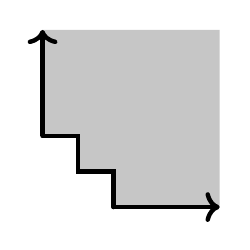
\begin{tikzpicture}[scale=.45]
  \path[fill=Gray!45] (5,0)--(2,0)--(2,1)--(1,1)--(1,2)--(0,2)--(0,5)--(5,5);
  \makegrid
  \draw[->, ultra thick] (2,0)--(5,0);
  \draw[-, cap=round,ultra thick] (2,0)--(2,1)--(1,1)--(1,2)--(0,2);
    \draw[->, ultra thick] (0,2)--(0,5);
  %\fill[Gray,fill=Gray] (-1,0) circle (6pt);
 % \fill[Gray,fill=Gray] (0,-1) circle (6pt);
\end{tikzpicture} \quad \quad
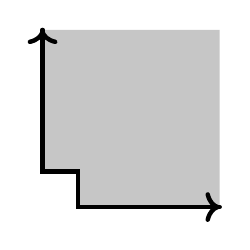
\begin{tikzpicture}[scale=.45]
  \path[fill=Gray!45] (5,0)--(1,0)--(1,1)--(0,1)--(0,5)--(5,5);
  \makegrid
  \draw[->, ultra thick] (2,0)--(5,0);
  \draw[-, cap=round,ultra thick]  (5,0)--(1,0)--(1,1)--(0,1)--(0,5);
    \draw[->, ultra thick] (0,2)--(0,5);
  %\fill[Gray,fill=Gray] (-1,0) circle (6pt);
 % \fill[Gray,fill=Gray] (0,-1) circle (6pt);
\end{tikzpicture} 
\caption{Left: The multigraded Castelnuovo--Mumford regularity of $\cO_{X}$ where $X\subset \PP^{1}\times \PP^{1}$ is the subschem of three points $([1:1],[1:4])$, $([1:2],[1:5])$, $([1:3],[1:6])$. Right: The multigraded Castelnuovo--Mumford regularity of $\cO_{\cH_{3}}$.}
\end{figure}
\end{center}

This project aims to deepen our understanding of multigraded regularity, its asymptotic behavior, and its relationship to the structure of free resolutions and positivity. 





%%%%%%%%%%%%%%%%%%%%%%%%%%%%%%%%%%%%%%%%%%%%%%%%%%%%%%%%%%%%%%%%%%%%%%%%%%%%%%%
 \subsection{Asymptotic Regularity of Powers of Ideals and Ideal Sheaves}
 %%%%%%%%%%%%%%%%%%%%%%%%%%%%%%%%%%%%%%%%%%%%%%%%%%%%%%%%%%%%%%%%%%%%%%%%%%%%%%%

 \begin{goal}
 	Let $X$ be a smooth projective toric variety with $S$ it's $\Pic(Y)$-graded Cox ring. Understand the asymptotic behavior of $\reg(I^p)$ and $\reg(\cI^p)$ where $I \subset S$ is an $\ZZ^r$-graded ideal and $\cI\subset \cO_{Y}$ is an ideal sheaf.
\end{goal}
 
 \begin{conjecture}\label{conj:reg-ideal-sheaves}
 	Let $Y$ be a smooth projective toric variety and $\cI \subset \cO_{Y}$ an ideal sheaf. With the notation as above:
	\[
	\lim_{p\to \infty} \frac{\reg\left(\cI^p\right)_{\RR}}{p} = \left\{ \; L \in \Pic(Y)_{\RR} \;\; \big| \;\; \pi^*(L)-E \text{ is nef on $\tilde{Y}$} \;\right\}.
	\]
 \end{conjecture}
 
 \begin{problem}
 	Prove Conjecture~\ref{conj:reg-ideal-sheaves}. 
 \end{problem}
 
  \begin{problem}
 	Is the Seshadri regions defined above be determined by the Newton-Okunkov body of some flag on $Y$. 
 \end{problem}
 
 \subsection{Bounds on Multigraded Regularity}
 
 \begin{problem}
 	Let $Y$ be a smooth projective toric variety with $S$ it's $\Pic(Y)$-graded Cox ring. If $I\subset S$ is a $\ZZ^r$-graded ideal bound the number of minimal generators of $\reg(I^p)$ as a function of $p$ in terms of invariants of $I$?
\end{problem}
 	
 \begin{problem}
 	Let $Y$ be a smooth projective toric variety and $Z\subset Y$ a smooth subvariety. Can one bound the multigraded regularity of $I_{Z}$ in terms of the codimension of $Z\subset Y$ and the degrees of minimal generators of $I_{Z}$?
\end{problem}

\begin{problem}
	Compute the multigraded regularity of torus invariant subvarieties of $Y$ in terms of the combinatorics of the cone defining them.
\end{problem}


Lastly as a somewhat losely connected project, I would like to explore the following specific example. The Deligne-Mumford moduli space of $n$-pointed stable curves of genus zero, denoted by $\overline{M}_{0,n}$, has long been of interest because of its rich geometry and combinatorics. Building upon work of Kapranov, Tevelev and Tevelev showed there is an embedding  $\Omega_{n}:\overline{M}_{0,n} \hookrightarrow \PP^{1}\times \PP^{2}\times \cdots \times \PP^{n-3}$, through which the log canonical embedding $\partial \overline{M}_{0,} + K_{\overline{M}_{0,n}}$ naturally factors. This embedding has been studied signficantly \juliette{fill in}, In particular, Monin and Rana produced a set of equations, arising as the $2\times 2$ minors of certain matrices of linear forms, the conjectured defined the scheme theoretic image of $\Omega_{n}$, this was recently prove true by Gillepsie, Griffin, and Levinson. This leads to the following natural question

\begin{problem}
 	Compute the multigraded Castelunovo--Mumford Regularity and minimal graded free resolution of the defining ideal of $\Omega_{n}(\overline{M}_{0,n}) \subset \PP^{1}\times \PP^{2}\times \cdots \times \PP^{n-3}$.
\end{problem}

Early explorations computing both the regularity and free resolution of $\Omega_{n}(\overline{M}_{0,n})$ for $n=4,5,6,7$ using \textit{Macaulay2} suggest, unsurprisingly, that both have significant NEDEDED. The proposed approach is two-fold: First, NEDEDED. Secondly, in order to produce the multigraded regularity of NEDEDEDED. Lastly, it is of interest to note that this NEDEDEDEDED

%%%%%%%%%%%%%%%%%%%%%%%%%%%%%%%%%%%%%%%%%%%%%%%%%%%%%%%%%%%%%%%%%%%%%%%%%%%%%%%
 \subsection{A Generalized Eisenbud--Goto Theorem for Toric Varieties}
 %%%%%%%%%%%%%%%%%%%%%%%%%%%%%%%%%%%%%%%%%%%%%%%%%%%%%%%%%%%%%%%%%%%%%%%%%%%%%%%

The relationship between Castelnuovo-Mumford regularity and the existence of linear resolutions is fundamental in classical commutative algebra. If a module $M$ over a standard graded polynomial ring is generated in degree $d$, then $M$ is $d$-regular if and only if it has a $d$-linear resolution (i.e., all entries in the matrices of the resolution are linear forms). In the multigraded setting of a toric variety $Y$, this equivalence breaks down dramatically. 

\begin{example}
In order to see the difference between linear and quasilinear resolutions we note that on a product of projective spaces the irrelevant ideal generally will have a quasilinear resolution, not a linear resolution.  For example, if we consider $\PP^{1}\times \PP^{2}$ so that $S=\KK[x_{0},x_{1},y_{0},y_{1},y_{2}]$ and $B=\langle x_{0},x_{1}\rangle\cap\langle y_{0},y_{1},y_{2}\rangle$ then the minimal graded free resolution of $S/B$ is: 
	\[\begin{tikzcd}[column sep=1.75em]
	S & \lar S(-1,-1)^6 & \lar
	  \begin{matrix}
	    S(-1,-2)^6\\[-3pt]
	    \oplus \\[-3pt]
	    S(-2,-1)^3
	  \end{matrix}
	  &
	  \lar
	  \begin{matrix}
	    S(-1,-3)^2\\[-3pt]
	    \oplus \\[-3pt]
	    S(-2,-2)^3
	  \end{matrix}
	  &\lar
	  S(-2,-3)
	  & \lar 0.
	\end{tikzcd}\]
In particular, we see that the minimal graded free resolution $S/B$ is not $(0,0)$-linear since $(-1,-1) \not\in L_1(0,0)$, however, it is $(0,0)$-quasilinear. Further, it is not the case that $M$ being $\dd$-regular implies $M_{\geq \dd}$ has a linear resolution \cite[Example 4.2]{bruceHellerSayrafi21}. 
\end{example}

The structure of the Cox ring $S$ and the geometry of the irrelevant ideal $B$ often obstruct the existence of linear resolutions. This necessitates weaker notions of linearity, such as quasi-linear resolutions, or the use of virtual resolutions . We seek to generalize the classical connections between regularity and resolutions to the multigraded setting.

 \begin{problem}\label{prob:eisenbud-goto}
 	Let $Y$ be a smooth projective toric variety with $S$ it's $\Pic(Y)$-graded Cox ring and $B$ its irelevant ideal. Let $M$ be a $\Pic(Y)$-graded $S$-module.  Find the correction generalization of $d$-quasi-linear resolution such that a $\Pic(Y)$-graded $S$-module  $M$ is $d$-regular if and only if the truncation $M_{\geq d}$ has a $d$-quasilinear resolution. 
\end{problem}

We propose that the constraints on the degrees of the resolution matrices should be dictated by the geometry of the nef cone $\Nef(Y)$ and the degrees of the generators of the irrelevant ideal $B$.

We will begin with the fundamental case of Hirzebruch surfaces $H_t$. The PI proposes the following conjecture, which  
 \begin{conjecture}\label{conj:eg-hirzebruch}
	Let $S$ be the $\ZZ^2$-graded Cox ring of the Hirzebruch surface $H_{t}$. If $M$ is a $\ZZ^2$-graded $S$-module then $M_{\geq d}$ has a $d$-linear resolution if and only if $d+\reg(S) \subset \reg(M)$. 
\end{conjecture}

\begin{problem}
	Prove Conjecture~\ref{conj:eg-hirzebruch}
\end{problem}
 
 While not equivalent to being regular, characterizing when $M_{\geq\dd}$ has a linear resolution in the traditional sense is still of interest algebraically. Using the same methods of controling the Betti numbers needed to answer Problem~\ref{prob:eisenbud-goto} would likely provide a way to give a cohomological characterization for when $M_{\geq\dd}$ has a linear resolution. 
 
\begin{problem}
 	Let $Y$ be a smooth projective toric variety with $S$ it's $\Pic(Y)$-graded Cox ring and $B$ its irrelevant ideal. Let $M$ be a $\Pic(Y)$-graded $S$-module.  Find a characterization for when the truncation $M_{\geq d}$ for $d\in \Pic(Y)$ has a linear resolution in terms of vanishing of the local cohomology groups $H^i_{B}(M)_{t}$. 
\end{problem}

Note the PI has provide an answer to this question when $Y$ is a product of proejctive spaces \juliette{CITATION}. 

Computing the regularity of a module $M$ directly from the definition is quite difficult as local cohomology computations tend to be slow in practice. Compute the truncation $M_{\geq \dd}$ and its associated minimal free resolution tends to be significantly quicker, and thus, Theorem~\juliette{ADD} and a resolution of Conjecture~\ref{conj:eg-hirzebruch} and Problem~\ref{prob:eisenbud-goto} provide a practical algorithm for checking whether a module is regular at a single multidegree $\dd\in \ZZ^r$. Finding an algorithm to compute all of the regularity region of $M$ remains an open question. 

\begin{problem}\label{prob:mg-reg-alg}
	Find an algorithm to compute a minimal generating set for $\reg(M)$. 
\end{problem}

Note this question is open in basically all cases except when $Y=\PP^n$, for example, even the case of $\PP^1\times \PP^1$ would be innovative. As right now even in these simple cases it requires quite a bit of ad hoc argument to showing that one has found all the minimal elements of $\reg(M)$. The difficulty to this is finding a box, in which one is guaranteed all the minimal generators of $\reg(M)$ live. Right now most bounds look like $L$-shaped regions, i.e. translates of $\Nef(X)$, which does not constraint the search space of minimal generators of $\reg(M)$. In this way finding an answer to Problem~\ref{prob:mg-reg-alg} is closely related to the question of questions around bounding multigraded regularity proposed in this project. 

Finally, as noted above, my previous work shows that the multigraded Betti numbers of a module do not determine its multigraded regularity. One might hope this can be saved by considering the multigraded Betti numbers of all virtual resolutions of $M$. A virtual resolution of a module $M$ is a free $\ZZ^r$-graded complex of $S$-modules with sheafifies to a resolution of $\tilde{M}$. 

\begin{problem}
	Let $Y$ be a smooth projective toric variety with $S$ it's $\Pic(Y)$-graded Cox ring and $B$ its irrelevant ideal. Let $M$ be a $\Pic(Y)$-graded $S$-module. Does the set of (multigraded) Betti numbers of all virtual resolutions of $M$ determine the multigraded regularity of $M$? 
\end{problem}

This question feels somewhat speculative, as I do not have a strong feeling for whether or not I believe it to be true. However, NEDEDEDEDDE

%%%%%%%%%%%%%%%%%%%%%%%%%%%%%%%%%%%%%%%%%%%%%%%%%%%%%%%%%%%%%%%%%%%%%%%%%%%%%%%
%%%%%%%%%%%%%%%%%%%%%%%%%%%%%%%%%%%%%%%%%%%%%%%%%%%%%%%%%%%%%%%%%%%%%%%%%%%%%%%
\section{Uniform Homological Algebra on Toric Varieties}\label{sec:uniform-homological-algebra-on-toric}
 %%%%%%%%%%%%%%%%%%%%%%%%%%%%%%%%%%%%%%%%%%%%%%%%%%%%%%%%%%%%%%%%%%%%%%%%%%%%%%%
%%%%%%%%%%%%%%%%%%%%%%%%%%%%%%%%%%%%%%%%%%%%%%%%%%%%%%%%%%%%%%%%%%%%%%%%%%%%%%%

This project aims to establish a uniform framework for studying homological invariants across different geometric realizations of the same Cox ring. A remarkable feature of toric geometry, arising from the construction of a toric variety as s GIT quotient, $Y=(\CC^n\setminus \VV(B))/(\CC^{\times})^r$, is that multiple toric varieties can have the same Cox ring $S$, as a graded ring, with the delineation between the different toric varieties only being captured by each variety having a different irrelevant ideal. Fixing a $\ZZ^r$-graded polynomial ring $S=\CC[x_1,\ldots,x_n]$ is equivalent to fixing a fan $\Sigma$ in $\RR^n$. The possible toric varieties with $S$ as it's Cox ring is governed by the second fan, also called the GKZ fan. 

Concretely the \juliette{ADDD} The choice of a chamber in $\Sigma_{\GKZ}$ can be thought of as specifying and of the following equivalent things: i) a toric variety $Y$ with Cox ring $S$, ii) an irrelevant ideal $B_{Y} \subset S$, iii) a stability condition \juliette{NNNEDED}. As described in \juliette{NDDD} the secondary fan also closely controls the birational geometry of a toric variety as when one moves between chambers the resulting toric varieties are related by birrational flips.  

It is a developing theme that many homological properties of toric varieties depend primarily on the underlying graded ring $S$, rather than the specific geometric realization $Y$. In particular, it seems like one NEDEDED We propose a uniform framework for studying homological algebra across all such varieties.

%%%%%%%%%%%%%%%%%%%%%%%%%%%%%%%%%%%%%%%%%%%%%%%%%%%%%%%%%%%%%%%%%%%%%%%%%%%%%%%
 \subsection{Regularity on the $D_{\Cox}$ Category}
 %%%%%%%%%%%%%%%%%%%%%%%%%%%%%%%%%%%%%%%%%%%%%%%%%%%%%%%%%%%%%%%%%%%%%%%%%%%%%%%


A recent instantiation of these ideas is the work of \juliette{cite} showing that birational variant of King's conjecture, on the existence of full strong exceptional collections of line bundles, is true if one is willing to work on a certain unifying derived category called $D_{\Cox}(X)$, called the Cox category of $X$. Roughly speaking the Cox category of $X$ is the smallest derived category containing the derived category $D(\cX_i)$ for each toric stack $\cX_i$ corresponding to maximal chambers in the secondary fan of $X$. While $D_{\Cox}(X)$ may \emph{not} be the derived category of any stack, it does have many nice properites. In particular

 \begin{problem}
 	Develop a theory of Castelunovo--Mumford regularity on the category $D_{\Cox}$ the restrict to the classical notion of regularity $Y_{i}$. 
 \end{problem}
 
 One natural approach to developing such a theory is to note that $D_{\Cox}(X)$ can be realized as an explicit full subcategory of $D(\tilde{\cX})$ where $\tilde{\cX}$ is any smooth toric stack with proper birational morphisms to the $\cX_i$. One could thus, hope to using the notion of multigraded regularity on $\tilde{\cX}$ and restrict it approaitely to the $D_{\Cox}(X)$ subcategory. A main obstruction to this is the choice of such a $\tilde{\cX}$ is not unique, and thus, defining regularity in this way may depend on the choice of $\tilde{\cX}$. 
 
I am proposing to circumventing this by noting there is natural construction of one such $\tilde{\cX}$ provided in \juliette{CITE}. Roughly speaking it is achived by building a toric stack via a combinatorial construction on each cone of the secondary fan of $X$. I believe that the stack resulting from this construction, while not unique to $D_{\Cox}(X)$ does seem to have nice universality properties. ADDDDD. 
 
 \begin{problem}
 	Characterize the ``uniqueness'' or ``universality'' of the $\cX_{\GKZ}$ stack construction.
 \end{problem}
 
 Proving a strong version of universality would provide a strong step towards defining regularity on $D_{\Cox}(X)$ via $D(\cX_{\GKZ})$ in a unique way.  As an effort in this direction, and with hopes to making expicit some of the steps of the construction provided in JULIETTE, I plan to implement the construction of the $\cX_{\GKZ}$ stack in \textit{Macaualay2}. 
 
\begin{problem}
	Implement the construction of the $\cX_{\GKZ}$ stack in the \textit{toricStacks} package being developed for \textit{Macaulay2} as part of \juliette{}
\end{problem}
 
 Work on this problem is currently on going with Maya Banks and John Cobb, and where have rough code that can compute $\cX_{\GKZ}$ in a narrow number of cases. We are working to expand its functionality. 
 
  %%%%%%%%%%%%%%%%%%%%%%%%%%%%%%%%%%%%%%%%%%%%%%%%%%%%%%%%%%%%%%%%%%%%%%%%%%%%%%%
 \subsection{Homological Invariants and Wall Crossings}
  %%%%%%%%%%%%%%%%%%%%%%%%%%%%%%%%%%%%%%%%%%%%%%%%%%%%%%%%%%%%%%%%%%%%%%%%%%%%%%%

 As the fan $\Sigma$ crosses a wall, the irrelevant ideal $B$ changes, leading to changes in the associated multigraded regularity and Betti numbers (since the notion of saturation changes). We aim to establish precise wall-crossing formulas that describe these changes.

 \begin{problem}
 	Let $I \subset S$ be a $\ZZ^r$-graded homogenous ideal. Let $Y$ and $Y'$ be toric varieties corresponding to two chambers $\Gamma, \Gamma' \subset \Sigma_{GKZ}$ that share a wall, with $B,B' \subset S$ the respective irrelevant ideals. Prove there exists a ``small'' subset $F \subset \ZZ^r$ depending only on $Y$ and $Y'$ such that:
	\[
	\reg_{Y}\left((J :_{S} B^{\infty})\right)+F =\reg_{Y'}\left((J :_{S} B'^{\infty})\right)+F.
	\]
 \end{problem}
 
 The subset $F$ represents a controlled shift in the regularity region. Proving this would establish that the homological complexity does not change arbitrarily under birational transformations, but rather follows predictable patterns dictated by the VGIT structure.


We also expect the minimal free resolutions of the saturated ideals to be closely related, particularly in the degrees corresponding to the "core" of the module that is unaffected by the change in saturation.

\begin{problem}\label{prob:wall-crossing-betti}
	With the set up as above, prove the minimal graded free $S$-resolutions of $(J :_{S} B^{\infty})$ and $(J :_{S} B'^{\infty})$ agree in small degree.
\end{problem}

The PI plans to use techniques from VGIT, the theory of derived equivalences induced by flops, and the study of local cohomology under changes of the irrelevant ideal to study these wall-crossing phenomena.


%%%%%%%%%%%%%%%%%%%%%%%%%%%%%%%%%%%%%%%%%%%%%%%%%%%%%%%%%%%%%%%%%%%%%%%%%%%%%%%
%%%%%%%%%%%%%%%%%%%%%%%%%%%%%%%%%%%%%%%%%%%%%%%%%%%%%%%%%%%%%%%%%%%%%%%%%%%%%%%
\section{Broader Impacts}\label{sec:broader-impacts} 
%%%%%%%%%%%%%%%%%%%%%%%%%%%%%%%%%%%%%%%%%%%%%%%%%%%%%%%%%%%%%%%%%%%%%%%%%%%%%%%
%%%%%%%%%%%%%%%%%%%%%%%%%%%%%%%%%%%%%%%%%%%%%%%%%%%%%%%%%%%%%%%%%%%%%%%%%%%%%%%

\subsection{Organizing} As discussed previously, I have organized 10+ national/international conferences, and I plan to continue organizing conferences at roughly this pace. Currently, I am organizing two research conferences in algebraic geometry \textit{Algebraic Geometry Northeastern Series (AGNES)} and \textit{BATMOBILE} both occurring in late 2024. I am also in the early stages of organizing an international workshop with Diane Maclagan on multigraded homological algebra and toric geometry, which I hope will occur in 2025. Tyler Kelly, Mike Hill, and I are also in the planning stages of organizing a satellite conference for LGBTQ+ mathematicians for the 2026 ICM in Philadelphia. 


The``GEMS'' workshop series that I co-founded sought to build a diverse community of mathematicians to address gender equity in the mathematical community from new perspectives. In particular, these conferences are indented to supplement the affinity group model of the \textit{Women in...} conference series by promoting broad conversations and networks. Going forward I am interested in expanding these ``GEMS'' workshops to other areas of mathematics and creating cross-field discussions that broaden the standard notion of gender equity in mathematics. In particular, there is a planned follow-up to \textit{GEMS in Commutative Algebra} scheduled for Fall 2025, and I am tentatively planning a version of \textit{GEMS in Algebraic Geometry} for 2026. As more of these conferences occur, I have plans to try to work with mathematicians in other fields to organize their own version of \textit{GEMS in...} conferences in their fields. 

When organizing these conferences I paid particular attention to making them as inclusive of women and non-binary researchers as possible. For example, I designed the registration form to be thoughtful of the concerns of transgender researchers and highlighted the locations of single occupancy and ADA-compliant restrooms. The importance of such efforts was highlighted by the following comment I received from a participant, ``I just wanted to thank you for making this workshop inclusive for people with all gender identifications. ... I have always felt out of place when I participated in conferences/workshops for women when they do not specify that non-binary people are welcome ... I really appreciate those questions you put in the registration form. It means a lot to me.'' I would like to work with various professional societies (AMS, AWM, NAM, Spectra, etc.) and research institutes (SLMath, ICERM, IAS, etc.) to produce a guide of best practices for organizing welcoming and inclusive mathematics conferences. By doing this I hope to make it easier for others to organize welcoming events. 

\subsection{ National \& International Advocacy.} I have worked with the Executive Committee of the \textit{Association for Women in Mathematics} to consider ways they could expand their support of women and non-binary mathematicians. I hope to continue this work and find further ways the AWM can support both women and non-binary mathematicians. Since Winter 2023 I joined SLMath's (formerly MSRI's)  \textit{Committee on Women in Mathematics}. I plan to remain on this committee until 2028 when my term is set to expire. In this role, I am hoping to organize a yearly retreat at SLMath that brings together small groups of 5-8 women (and underrepresented individuals more generally) who have been implementing innovative ideas promoting equity in mathematics and brainstorm ways to scale their efforts and effect radical positive change for women in mathematics.  


\subsection{A More Inclusive Learning Community.}  Going forward I am excited to continue my work supporting LGBTQ+ students, and would love to continue building organizations to do so. In particular, given the amazing successes of programs like MSRI-UP and the EDGE Program, I would love to organize a summer REU program specifically aimed at supporting and promoting LGBTQ+ mathematicians. Further, I am in the early stages of planning a mentorship program to help guide LGBTQ+ undergraduates through the process of applying to graduate programs in mathematics and helping young LGBTQ+ graduate students establish themselves. The plan would be to break participants into groups with each group having LGBTQ+ mathematicians at various career stages, thus allowing participants to exchange advice, find support, and build mentoring networks.

\subsection{Mentoring.} As a new faculty member at Dartmouth College I hope to continue and expand the mentoring I do with students, continuing a focus on mentoring students from underrepresented groups. Since arriving on campus in the late Summer I have begun mentoring one graduate student and one undergraduate woman. While still early it seems likely that I will end up co-advising the graduate student and advising the undergraduate's senior thesis. I am also working with the college's AWM Student Chapter and the Out in STEM Student Chapter. 


\newpage
\renewcommand{\bibliofont}{\normalsize}
%%%%%%%%%%%%%%%%%%%%%%%%%%%%%%%%%%%%%%%%%%%%%%%%%%%%%%%%%%%%%%%%%%%%%%%%%%%%%%%%%%%%%%%%%%%%%%%%%%%%%%%%%%
\bibliographystyle{alpha}
\bibliography{sample}

%%%%%%%%%%%%%%%%%%%%%%%%%%%%%%%%%%%%%%%%%%%%%%%%%%%%%%%%%%%%%%%%%%%%%%%%%%%%%%%%%%%%%%%%%%%%%%%%%%%%%%%%%%

\end{document}